%\section{Coping with Cross Traffic}
\section{\cut{Handling }Unfavorable Conditions}\label{s:queue-ctl}

Recall from \S\ref{s:deploy} that \name can reliably shift queue build up from the bottleneck to itself when, (a) the cross-traffic is not buffer-filling, and (b) all of its component traffic shares the same bottleneck in the network.
In practice, either of these conditions may break. 
%not always hold on the real Internet, and they may change over time.
In this section, we describe how \name can re-use the same measurements from \S\ref{s:measurement} to detect when these conditions do not hold. In such cases, \name (temporarily) disables its rate limiting (falling back to status-quo performance) until favorable conditions arise again. 
%Thus, even in the worst case \name will not degrade performance (relative to the status quo without \name).
% simply degrades to status quo performance.
% Of course, in real Internet conditions, there may be scenarios where these conditions do not hold.
% In these cases, \name gracefully degrades to status quo performance. 

\subsection{Buffer-Filling Cross Traffic}
\label{s:buffer-filling}

%%%%%%%%%%%%%%%%%%%%%%%%%%%%%%%%%

% As described in \S\ref{4.3}, \name uses a delay-based congestion control algorithm to control queues in the middle of the network. 
It is well known that delay-based congestion control algorithms (as \name uses) lose throughput when competing with buffer-filling algorithms~\cite{copa}.\pg{cite nimbus as well} 
% However, it is well-known that such algorithms lose throughput when competing with buffer-filling algorithms~\cite{copa}.
% Therefore, in order to compete fairly with buffer-filling cross-traffic, \name must first detect the presence of such traffic and disable its use of a delay-based controller.
To prevent this, \name utilizes prior work, Nimbus~\cite{nimbus-arxiv}, which provides a mechanism for detecting the presence of buffer-filling cross traffic,\footnote{In particular, Nimbus actually detects ``elastic'' traffic (defined in~\cite{nimbus-arxiv}), which includes, but is not limited to, buffer-filling traffic. \cite{nimbus-arxiv} provides an explanation of this distinction and a justification that it is a reasonable approach.}
and proposes temporarily switching to a buffer-filling scheme to compete fairly whenever such cross traffic is present.
% and proposes switching between two modes: using a buffer-filling scheme when buffer-filling cross traffic is present and using a delay-control scheme otherwise.
At a high-level, the detection mechanism works as follows: given a desired sending rate $r(t)$ (computed according to the underlying congestion control algorithm), Nimbus superimposes an asymmetric sinusoid onto $r(t)$ to compute the actual sending rate. Then, it monitors the ACK receive rate in the frequency domain\pg{it uses the send and receive rate to compute cross-traffic rate, it monitors cross-traffic rate in the frequency domain}; the sinusoidal variations in the sending rate will be visible in the receive rate\pg{cross-traffic rate} only if some buffer-filling cross traffic is sharing the same bottleneck queue.%  buffer-filling cross traffic will cause an ``echo'' of these variations in the receive rate, while non-buffer-filling traffic will not.
\footnote{\cite{nimbus-arxiv} includes a detailed evaluation of Nimbus' accuracy of detecting elastic cross traffic and speed of switching between the two modes, using both emulated and real-world experiments. \name{}'s use of Nimbus does not impact its accuracy or speed of switching.}

But what exactly should the \inbox do when it detects buffer-filling traffic? Using a buffer-filling scheme for the bundle as in Nimbus would be fraught: since a bundle is comprised of many individual flows, the \inbox would need to know the number of flows in the bundle to know how aggressively it should compete in order to receive its fair share (as in the status quo)~\cite{multcp}. Especially on high-performance datapaths this number may vary significantly over time and would be difficult to measure~\cite{heavy-hitters}.
% to use a buffer-filling scheme for the bundle, \name{} would need to 
% But what exactly should the \inbox do when it detects this condition?
% A naive approach might replace the delay-based control at \name with a loss-based buffer-filling congestion control such as Cubic. 
% However, with this approach, \name must 
% in order to know the fair share of throughput that the component flows measure the number of flows in a bundle in order to compete as aggressively in proportion to achieve an aggregate throughput equivalent to the status quo~\cite{multcp}. Especially on high-performance datapaths, this number may vary significantly over time and be difficult to measure~\cite{heavy-hitters}.

Instead, we propose a simpler solution.
Since each connection in a bundle is already employing their own congestion controllers, \name{} can simply \emph{let the traffic pass}, \ie{} increase the pacing rate at the \inbox to stop controlling queues.
% Since the bundleach employing their own congestion controllers, \name can simply \emph{let the traffic pass}, \ie increase the pacing rate at the \inbox to stop controlling queues.
Then, the end-host congestion control loops will naturally compete fairly with the buffer-filling cross traffic, just as they would without \name{}.

However, letting the traffic pass creates a new challenge. 
In order to determine when it is safe to resume delay-control while in buffer-filling mode, Nimbus must superimpose the sinusoid in both modes. But if we let the traffic pass, the \inbox queue will never build and thus there will not be sufficient packets in the queue to satisfy the momentary rate increases necessary for the up-pulse. Without this, once the \inbox{} switches to the buffer-filling mode, it would not be able to gather sufficient information to switch back to delay-control mode.

%\paragrapha{Active Probing}
% This brings us to the next natural question: how can the \inbox know when it is safe to resume delay-control (and scheduling) after disabling it?
%It is important to distinguish between \emph{self-inflicted} queueing delay and queueing delay due to cross traffic.
%When the queueing delay is purely self-inflicted, it is safe to resume control over the queues at the \inbox.
% One approach is to send passive probes along the network to detect the presence/absence of queuing. However, such passive measurements cannot distinguish between the self-inflicted queuing due to \name's traffic and the queuing due to cross-traffic. If the bottleneck queue is entirely self-inflicted, it is safe (and desirable) to resume delay-control and scheduling.
%Passive probing is insufficient to determine this state, since passive measurements of the bottleneck will be identical in the case of self-inflicted queueing and queueing driven by cross traffic.
% Therefore, it is important to \emph{actively probe}, that is, change the rate of bundled traffic and observe the response of the cross traffic. 
% This is exactly what the Nimbus mechanism does.
% At a high level,
% TODO: r(t) is the desired sending rate, A sint is super-imposed on top
% r(t) is the rate you are trying 
% something calculates r(t), calculate based on sending and receiving rate, using e.g. basic delay rule  
% now we are trying to deicde, when we want to let the pas
% we are trying to figure out the change to r(t) from the basic delay rule
% if its too large you'll converge too quickly and cant superimpose sinusoid on top of it
% given a desired sending rate $r(t)$, Nimbus superimposes an asymmetric sinusoid on top of $r(t)$, and measures the cross traffic's response in the frequency domain.
% Nimbus sinusoidally varies the sending rate $r(t) = A sin(\frac{4\pi{}t}{T})$ during the up-pulse, where $A$ is the pulse amplitude (set to one-fourth of the estimated bottleneck bandwidth) and $T$ is the pulse duration, and measures the cross traffic's response in the frequency domain.
% The \inbox can use the Nimbus algorithm to detect when to relinquish control over the queue by interposing this sending pattern over the delay-controller's rate decisions.
% However, if the \inbox entirely drains its queues into the network, it will no longer be possible for Nimbus to overlay pulses onto the traffic pattern, and it will be unable to determine the nature of the cross traffic.
% Practically, this would mean that once \inbox switches to compete with cross traffic, it would never gain the information necessary to switch back.

In order to support the Nimbus pulses while also letting the traffic pass,
% Instead, to support active probing while also letting the traffic pass,
the \inbox must maintain sufficient queueing for the up-pulse,
%queueing.
% How many packets should this be? The \inbox should be able to generate enough packets for the up-pulse,
\ie the area under the up-pulse curve: 
$A \int_0^{\frac{T}{4}} \sin(\frac{4\pi{}t}{T}) dt = \frac{AT}{2\pi}$.
From \cite{nimbus-arxiv}, we use $T = 0.2$ seconds and $A =$ one-fourth the bottleneck bandwidth. Then, by Little's law, the amount of extra queueing necessary is equivalent to
% By Little's law, we can calculate the amount of extra queueing: 
$\frac{T}{8\pi}$, or $8$ms. \pg{why by little's law, you just substituted value of A as $\mu/4$.}% We call this the target queueing delay, or $q_T$. 
We thus configure the \inbox to maintain a target queueing delay of $q_T = 10$ms (the additional $2$ms is a cushion against input variance).\footnote{This extra queueing is in addition to normal queueing in the network. As a result, the end-to-end connections will see mild RTT inflation, but in \S\ref{s:robust:cross} we show that this effect is not large; \name still achieves performance comparable to the status quo.}

% In order to achieve this target queueing delay,
Of course, while any additional delay beyond $q_T$ would provide sufficient queue for the up-pulse, it would also add unnecessary delay to the end-to-end connections. Thus, we want to stay as close to $q_T$ as possible. In order to achieve this,
we design a PI controller for the \inbox which determines how the base sending rate $r(t)$ should be updated\footnote{Note that $\dot{r}(t)$ is an update to the base sending rate \emph{before} superimposing the Nimbus pulse.}
at each time step to move to the target:\footnote{This is similar to the PIE AQM mechanism~\cite{pie}, however, unlike PIE, there is no feedback delay between setting $r(t)$ and observing its effect on $q(t)$.}
$\dot{r}(t) = \alpha (q(t) - q_T) + \beta (\dot{q}(t))$, where $q(t)$ is the current queue size at the \inbox in ms and $\alpha$ and $\beta$ are both positive.
If the current queueing delay is greater than the target, the first term will be positive, causing the rate to increase, and the queue to drain faster, ultimately decreasing the queueing delay. Similarly, if the queue size is growing, the second term will be positive and again ultimately decrease the queueing delay\pg{don't call it queueing delay, queueing target values in ms is assuming the bottleneck bandwidth rate, not r(t).}. The scale of $\alpha$ and $\beta$ represent a tradeoff: the larger they are, the faster the controller will approach the target queueing delay. If they are too large, the controller's variations will nullify the Nimbus pulse. If they are too small, it will take too long to reach the target delay. Experimentally, we found that $\alpha=10$ and $\beta = 10$ provide a good balance for the types of scenarios included in our evaluation and thus used these values for all of our experiments.


% This problem is similar to the role of the PIE AQM mechanism~\cite{pie}, which also seeks to maintain a queueing delay target.
% Correspondingly, we design a PI controller at the \inbox as part of the fairness control module. 
% It overlays a rate $r$ corresponding to , where $q$ is the queue size and $q_T$ is the target queue size computed above.
% We pick $\alpha = 10$ and $\beta = 10$ by solving for a convergence time of one RTT (Appendix~\ref{app:derive-ab}).
% as per \S\ref{s:qctl:pi}.

\subsection{Imbalanced Multipathing}\label{s:queue-ctl:ecmp}
Since a \bundle contains many component connections, a load balancer may send them along different paths. If the load along different paths is well-balanced, \name will accurately treat a load-balanced bottleneck link as a single link whose rate is the sum of the rates of each sub-link. However, when the load along different paths is imbalanced, the series of measurements \name collects will be a random sampling of the different paths, which would confuse the delay-control algorithm and cause it to perform poorly. Fortunately, such cases are straight-forward to detect with our measurement technique. 
More specifically, load imbalance will result in many epoch measure packets arriving out-of-order at the \outbox (whenever epoch packet $i$ happens to traverse a path with a larger delay than epoch packet $i+1$), and consequently, out-of-order ``congestion ACKs'' at the \inbox.  Figure~\ref{fig:queue-ctl:ecmp:motivation} demonstrates this in an emulated imbalance scenario. 

Therefore, we use the fraction of epoch measurement packets that arrive out-of-order as an indicator of load imbalance due to multipathing.
If this number is small, the links are roughly balanced and \name will operate as expected.
If it is large, it indicates load imbalance, in which case \name's rate control may not work well. 
%While we believe that it is possible to design a rate controller that distinguishes RTT samples from different paths, and computes appropriate aggregate rates, we leave this for future research, and instead adopt a simpler
%the delay controller will make erratic adjustments as it briefly observes high RTTs, and may lose throughput as a result.
In \S\ref{s:eval:ecmp}, we experimentally determine an out-of-order fraction of 5\% to be a good threshold indicating whether or not the links are balanced: all single-path scenarios resulted in an order of magnitude fewer out-of-order packets, and all multi-path scenarios resulted in an order of magnitude greater.

% Therefore, if the reordering level is above 5\%, we disable rate control and revert to status quo performance. We evaluate this approach (and justify our chosen threshold) in \S\ref{s:eval:ecmp}.
%In this case, the measurement sub-system (\S\ref{s:measurement}) would report erratic measurements corresponding in turn to each of the possible paths.
% To see why, consider that \name's epoch-based rate measurements do not distinguish the path the packets take, and instead consider only the number of packets sent and received in an epoch.
% Thus, \name will accurately measure a load-balanced bottleneck link as a single link with the aggregate rate of each sub-link.
% However, for RTT measurements, the link with the lowest RTT will be over-sampled because the first epoch feedback packet to arrive will be from this link.
% So, \name will not detect building queues in other links.
% In most cases, this is not fatal: the delay controller might yield too much queue to the bottleneck, causing \name to miss out on performance improvements.
% We leave the design of a delay controller that does not over-react to conflicting measurements, and thus further optimizes traffic-control ability, to future work.

%In extreme cases, there may be persistent imbalance in the level of queueing. 
\begin{figure}
    \centering
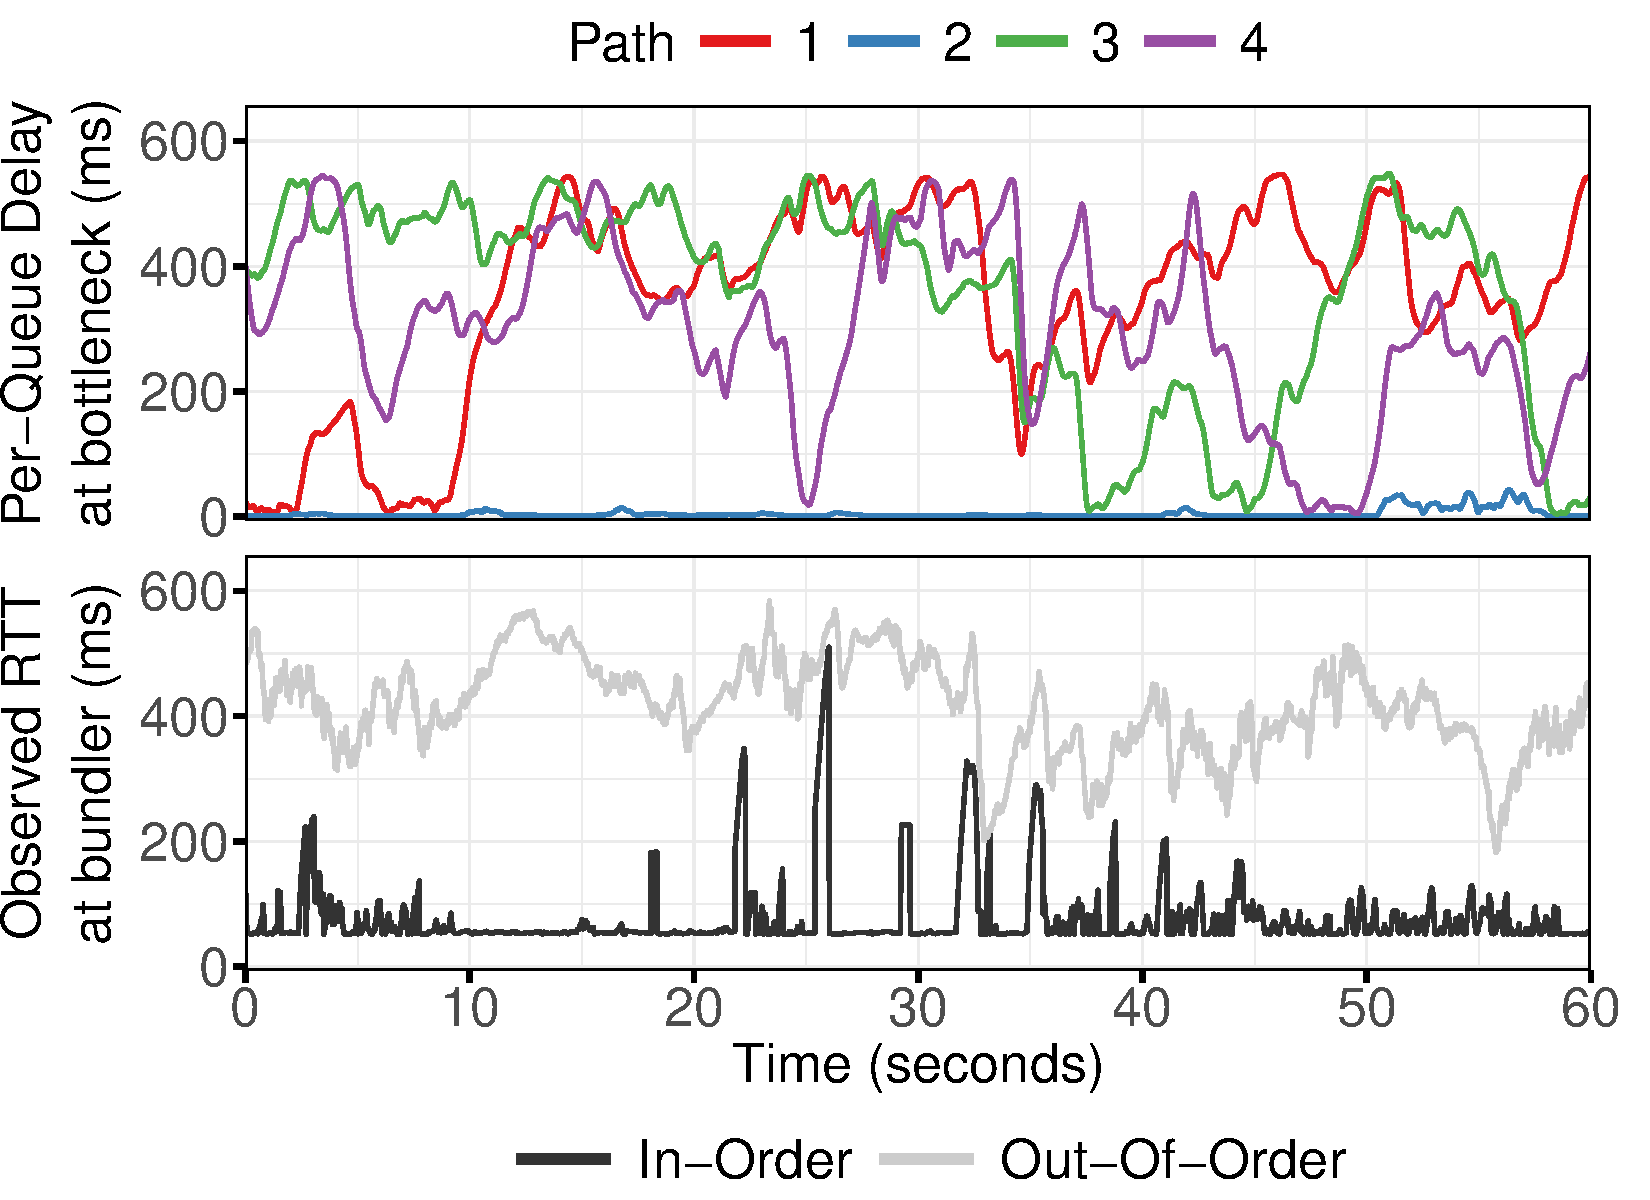
\includegraphics[width=\maxwidth]{figure/ecmp_delay.pdf} 
\vspace{2pt}
\caption{(Top) True delay for all packets of \name's component flows based on which of 4 load-balanced paths they traversed (unknown to \name). (Bottom) Delay measurements observed by Bundler, colored based on whether they were derived from an in-order or out-of-order epoch packet. Bundler's measurements cannot distinguish how many paths there are, but the relative number of out-of-order measurements is enough to clearly indicate the presence of multiple RTT-imbalanced paths.}
\label{fig:queue-ctl:ecmp:motivation}
\end{figure}

